%!TEX root = ../main.tex



\section{Η έννοια της ανάλυσης}

\lettrine[findent=2pt]{\fbox{\textbf{Κ}}}{ατά} την αποτύπωση οποιουδήποτε αναλογικού σήματος $S(t)$ σε ψηφιακή μορφή $S_i$, πραγματοποιείται μια διαδικασία που ονομάζεται \emph{δειγματοληψία (sampling)} κατά την οποία ένα συνεχές σήμα γίνεται διακριτό και στη συνέχεια εφαρμόζουμε \emph{κβαντισμό} στις τιμές του, για να περάσουμε σε ψηφιακή αναπαράσταση. Όπως φαίνεται και στο σχήμα \ref{fig:sampling}, σε διακριτές χρονικές στιγμές λαμβάνουμε την τιμή του αναλογικού σήματος (μέσω ενός μετατροπέα Αναλογικού σε Ψηφιακό (ADC)) κι έτσι δημιουργούμε μια σειρά από τιμές (\emph{δείγματα}) τα οποία έχουν συγκεκριμένη και σταθερή χρονική απόσταση $T_s$. Η χρονική απόσταση έχει νόημα μόνο ως προς το αναλογικό σήμα, ενώ στην ψηφιακή μορφή των δειγμάτων αναφερόμαστε σε αυτά με ένα δείκτη $n$ και μεταξύ αναλογικού και ψηφιακού σήματος ισχύει ότι $S_i=S(nT_s)$.
\begin{figure}[h]
  \centering
  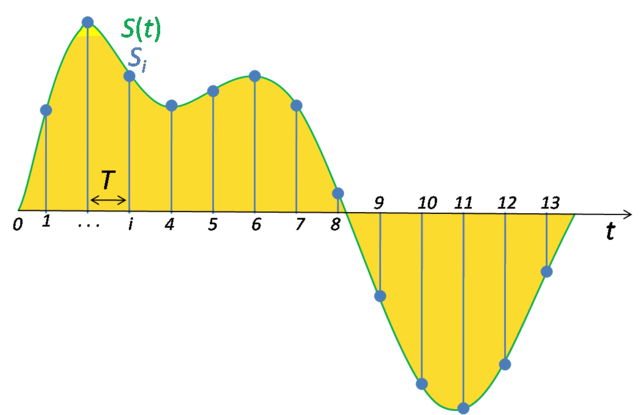
\includegraphics[width=0.6\textwidth]{Signal_Sampling}
  \caption{Δειγματοληψία ενός αναλογικού σήματος}
  \label{fig:sampling}
\end{figure}
Κατά τη δειγματοληψία ``χάνουμε'' αρκετή από την πληροφορία που περιέχει το αναλογικό σήμα, καθώς οι τιμές που βρίσκονται μεταξύ των διαστημάτων $T_s$ όπου λαμβάνουμε δείγματα δε λαμβάνονται υπόψη. Ακόμη, λόγω της πεπερασμένης ακρίβειας των ψηφιακών συστημάτων για αναπαράσταση αριθμών, η τιμή που έχει το σήμα στρογγυλοποιείται στην πλησιέστερη (είτε μεγαλύτερη είτε μικρότερη) τιμή που μπορεί να αναπαραστήσει το σύστημά μας.

Όπως γίνεται αντιληπτό, σε πολλές των περιπτώσεων η δειγματοληψία μπορεί να έχει καταστροφικές συνέπειες για το αναλογικό σήμα. Ωστόσο, υπό προϋποθέσεις, μπορεί να είναι αντιστρεπτή διαδικασία -- μπορούμε δηλαδή από τα δείγματα που έχουμε λάβει να επιστρέψουμε στην αναλογική μορφή του σήματος. Οι προϋποθέσεις αυτές ορίζονται από το θεώρημα \emph{Shannon-Nyquist} (\ref{thrm:shannon-nyquist}), ως:
\\
\begin{theorem}[Shannon-Nyquist]
	\label{thrm:shannon-nyquist}
	Ένα σήμα με μέγιστη συχνότητα $f_{max}$ μπορεί να ανακτηθεί από τα δείγματά του, αν αυτά ληφθούν με συχνότητα $f_s>2f_{max}$, ή αλλιώς με περίοδο $T_s<\frac{1}{2f_{max}}$. \cite{proakis_sampling}
\end{theorem}